\documentclass[12pt]{article}

\title{Visualizing the escape paths of quaternion fractals}
\author{S. Halayka\footnote{sjhalayka@gmail.com}}
\date{\today}
\usepackage{listings}
\usepackage{xcolor}

\usepackage{graphicx}
\usepackage{setspace}
\usepackage{amsmath}
\usepackage{url}
\usepackage[margin=1in]{geometry}
\begin{document}


%\doublespace


\maketitle

\begin{abstract}
The escape paths of the points in some quaternion fractal sets are visualized using OpenGL. C++ source code is provided.
\end{abstract}


\section{Escape paths that do not reach infinity}

As discussed in \cite{halayka}, a 3D scalar field of quaternion magnitudes (e.g. $|Z|$) results from calculating a quaternion fractal set when using a finite 3D lattice of regularly spaced points as input.

Here we will visualize the escape paths, using OpenGL, for those points that maintain a quaternion magnitude less than the infinity threshold value (e.g. $4.0$) during the iteration process (e.g. $8$ iterations).

The notion that the escape paths can make for nice visualizations was independently found by Paul Bourke \cite{bourke}.
Bourke's work was inspired by the Buddhabrot.
Bourke's work focuses on the escape paths that reach infinity, whereas here we will focus on escape paths that do not reach infinity.

Here we will use Bezier curves and cylinders to draw the escape paths.

The length of these `shaggy' escape paths will be shortened to only $20\%$ of the total length, giving the impression of an isotropic buzz cut.

The C++ code for this paper can be found at \cite{halayka2}.

\lstset { %
    language=C++,
    backgroundcolor=\color{black!5}, % set backgroundcolor
    basicstyle=\footnotesize,% basic font setting
}

\begin{lstlisting}
vector_3 getBezierPoint(vector<vector_3> points, float t)
{
	int i = points.size() - 1;

	while (i > 0)
	{
		for (int k = 0; k < i; k++)
		{
			points[k].x += t * (points[k + 1].x - points[k].x);
			points[k].y += t * (points[k + 1].y - points[k].y);
			points[k].z += t * (points[k + 1].z - points[k].z);
		}

		i--;
	}

	return points[0];
}
\end{lstlisting}

\begin{lstlisting}
vector_3 line = pos[i][j + 1] - pos[i][j];
			
glPushMatrix();
glTranslatef(pos[i][j].x, pos[i][j].y, pos[i][j].z);

float line_len = line.length();
line.normalize();
			
float yaw = 0.0f;

if (fabsf(line.x) < 0.00001 && fabsf(line.z) < 0.00001)
	yaw = 0.0f;
else
	yaw = atan2f(line.x, line.z);

float pitch = -atan2f(line.y, sqrt(line.x*line.x + line.z*line.z));

glRotatef(yaw*rad_to_deg, 0.0f, 1.0f, 0.0f);
glRotatef(pitch*rad_to_deg, 1.0f, 0.0f, 0.0f);

gluCylinder(glu_obj, 0.005, 0.005, line_len, 20, 2);

glPopMatrix();
\end{lstlisting}




%\begin{figure} 
%  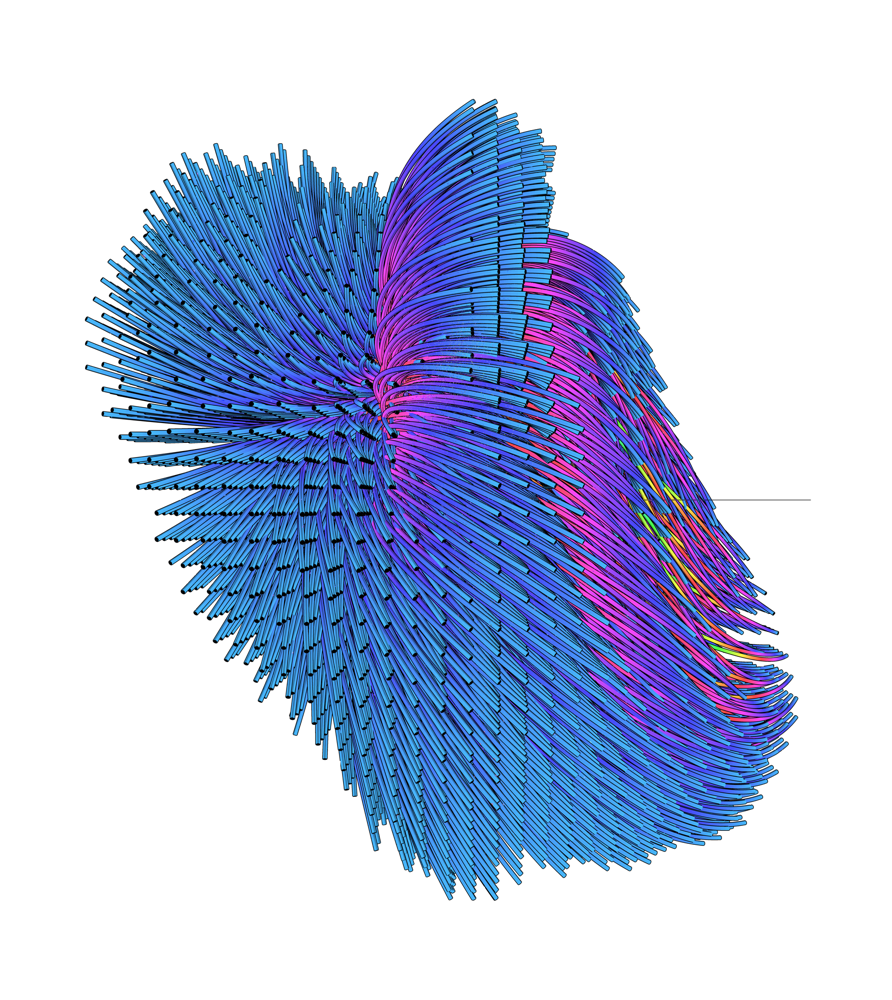
\includegraphics[width=\textwidth]{1.png}	
%  \caption{$Z' = Z^2 + C$, where $C_{xyzw} = 0.3, 0.5, 0.4, 0.2$.}
%\end{figure}

%\begin{figure} 
%  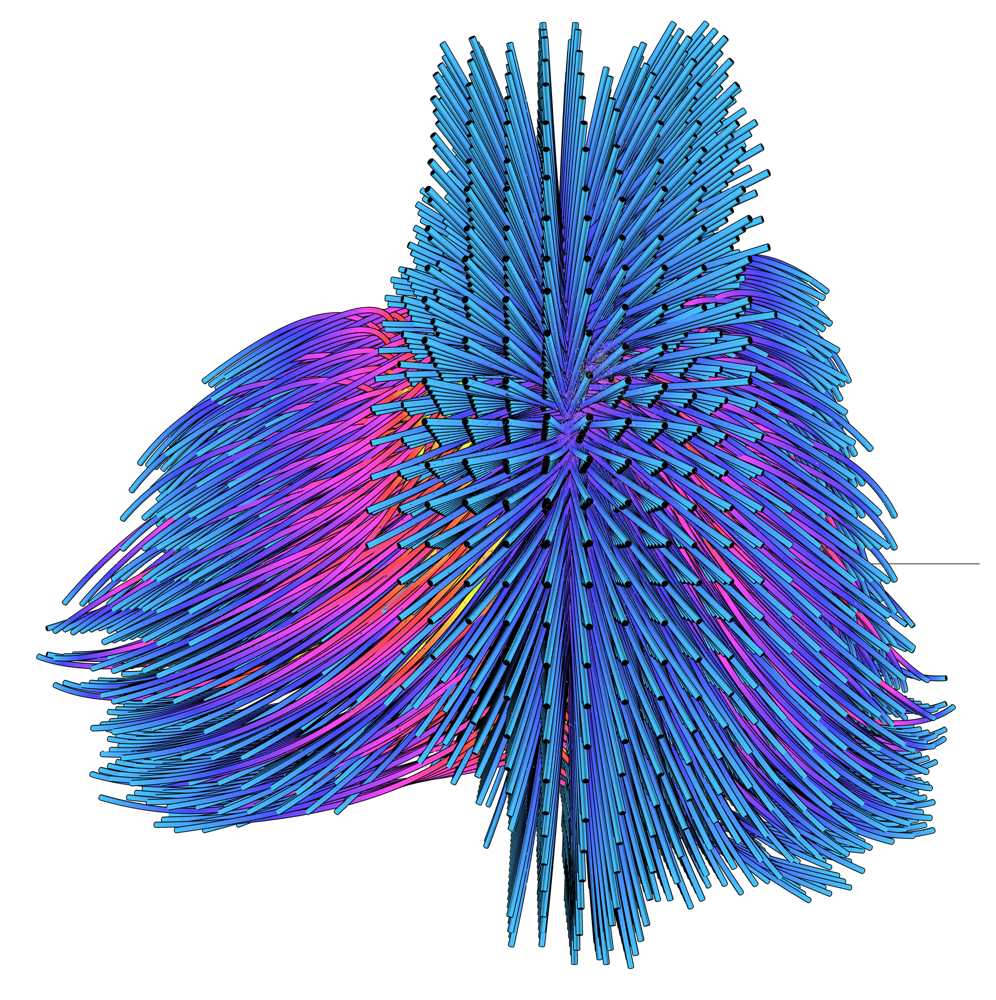
\includegraphics[width=\textwidth]{2.png}	
%  \caption{$Z' = Z^3 + C$, where $C_{xyzw} = 0.3, 0.5, 0.4, 0.2$.}
%\end{figure}

\begin{figure} 
  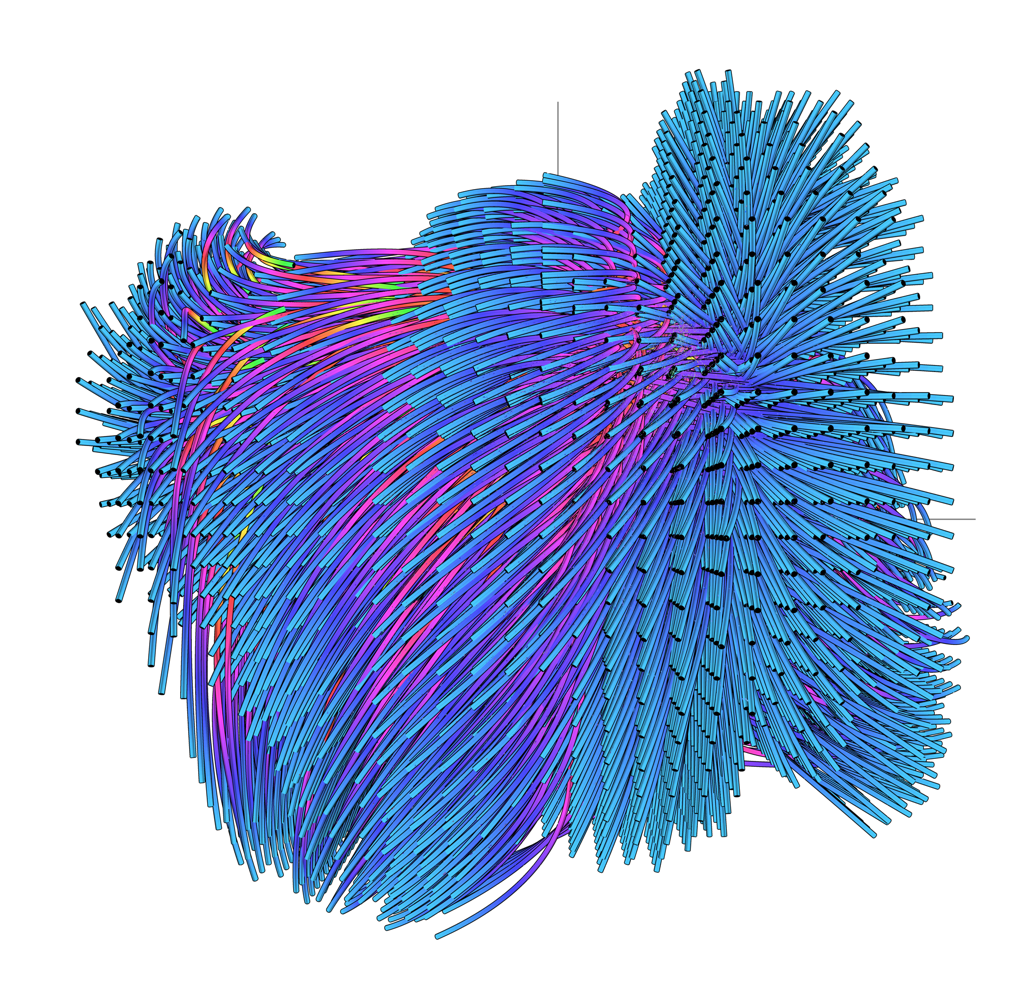
\includegraphics[width=\textwidth]{3.png}	
  \caption{`Pinhead': $Z^{\prime} = Z^4 + C$, where $C_{xyzw} = 0.3, 0.5, 0.4, 0.2$.}
\end{figure}

%\begin{figure} 
%  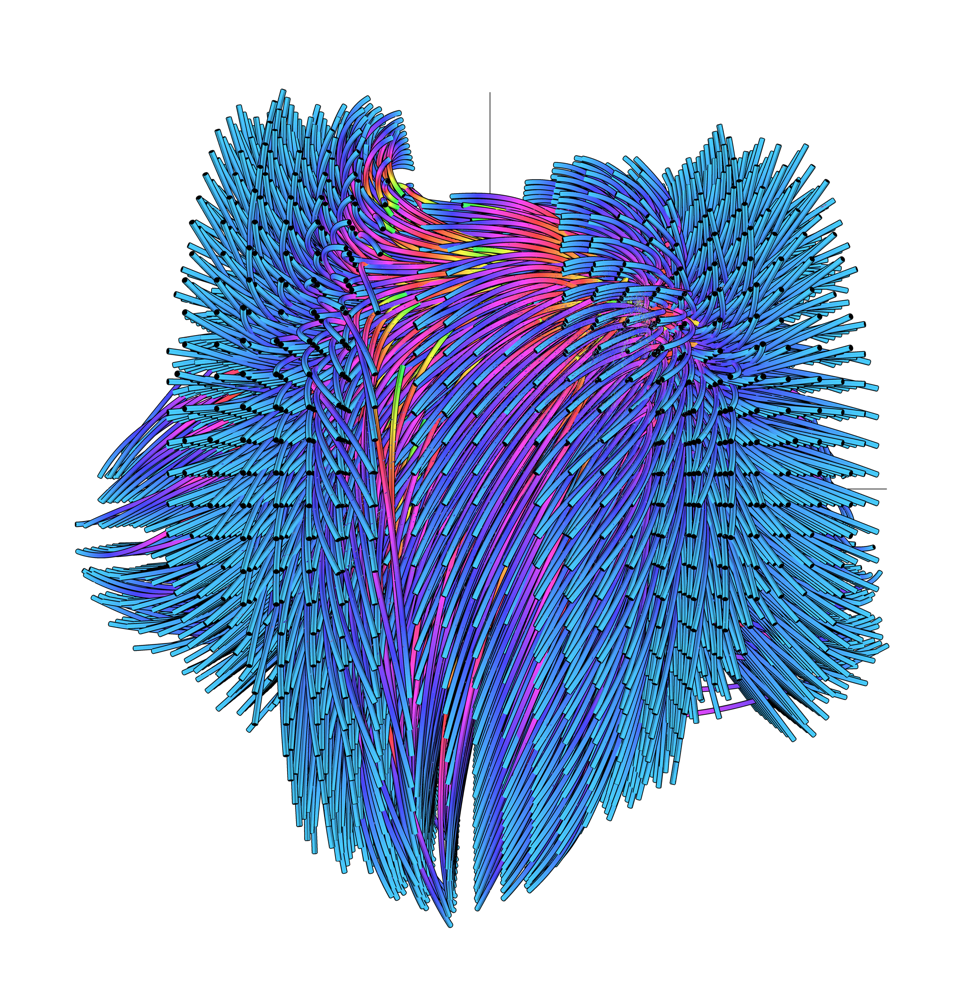
\includegraphics[width=\textwidth]{4.png}	
%  \caption{$Z' = Z^5 + C$ , where $C_{xyzw} = 0.3, 0.5, 0.4, 0.2$.}
%\end{figure}

%\begin{figure} 
%  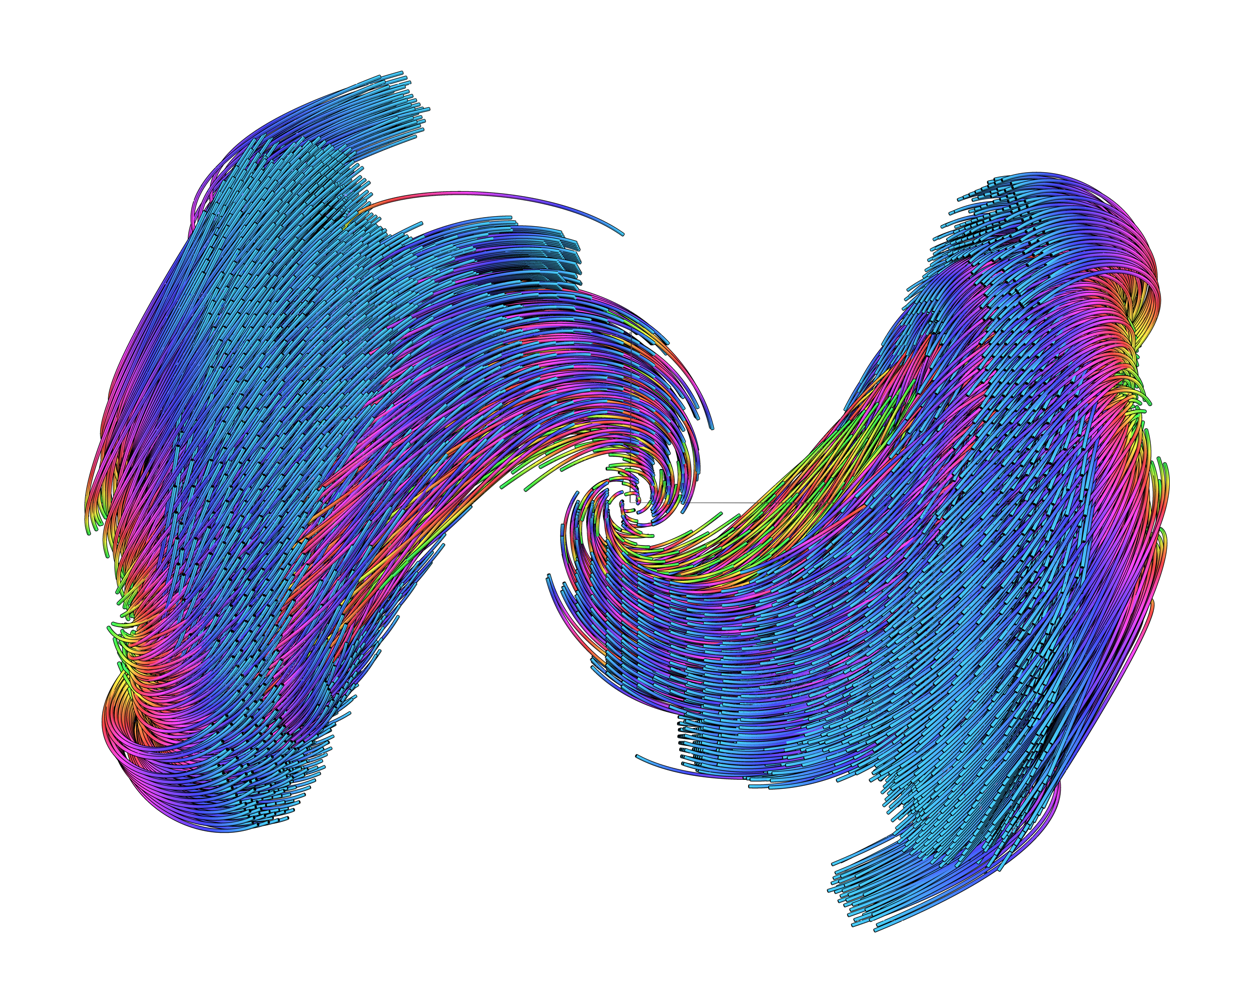
\includegraphics[width=\textwidth]{5.png}	
%  \caption{$Z' = \sin(Z) + C\cdot\sin(Z)$, where $C_{xyzw} = 0.3, 0.5, 0.4, 0.2$.}
%\end{figure}
 

\pagebreak

\begin{thebibliography}{9}

\bibitem{halayka} Halayka S. \emph{Some visually interesting non-standard quaternion fractal sets} Chaos, Solitons \& Fractals Vol. 41, Issue 5		

\bibitem{bourke} \url{http://paulbourke.net/fractals/trajectories/}

\bibitem{halayka2} \url{https://github.com/sjhalayka/bezier_fractal}

\end{thebibliography}


\end{document}

